\chapter{Method}
\thispagestyle{empty}
In this chapter, various methods involved in this project are explained. They are arranged in the way that is corresponding to the four tasks.
\section{Environment}
\begin{figure}[t]
	\begin{center}
		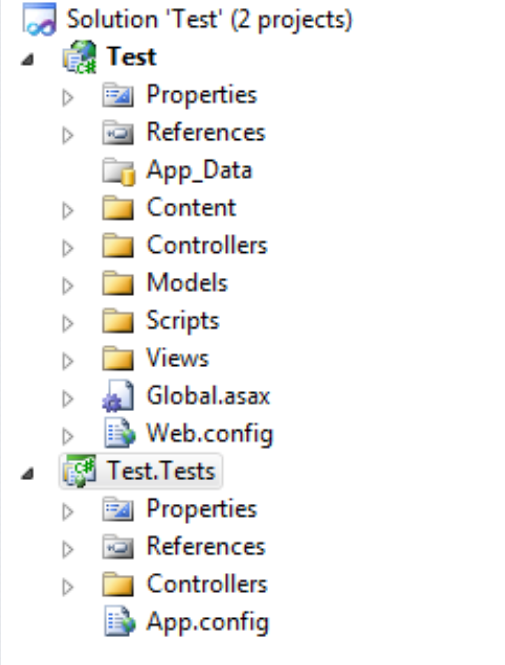
\includegraphics[scale=0.4]{mvcOriginalLayout.png}
	\end{center}
	\caption{MVC layout.}
	\label{fig:mvc_layout}
\end{figure}
\subsection{Visual Studio}
While working with Visual Studio, developers should keep one thing in mind, that there is only one solution at one time, and this solution will always
have one or more projects \cite{vs_book}. This might feel a little bit strange for new users, but it is quite reasonable if one thinks about this 
organization especially when one task is too complicated and immense to fit in as one project.

This project is based on the ASP.NET MVC Web Application technology. While creating one such application with Visual Studio, it automatically adds a 
number of files and directories to the project, as is shown in Figure~\ref{fig:mvc_layout}. Although this project is based on one existing project 
(no need to create new project), understanding the file organization is critical, for the existing project keeps the original layout somehow.

One new ASP.NET MVC project by default has six top-level directories: \cite{mvc_folder_layout}
\begin{table}[h]
	\begin{tabularx}{\textwidth}{| l | X |}
		\hline
		/Controllers & Where we put Controller classes that handle URL requests \\
		\hline
		/Models & Where we put classes that represent and manipulate data \\
		\hline
		/Views & Where we put UI template files that are responsible for rendering output \\
		\hline
		/Scripts & Where we put JavaScript library files and scripts (.js) \\
		\hline
		/Content & Where we put CSS and image files, and other non-dynamic/non-JavaScript content \\
		\hline
		/App\_Data & Where we store data files we want to read/write. \\
		\hline
	\end{tabularx}
	\caption{File organization.}
\end{table}

ASP.NET MVC does not require this structure. However, developers working on large applications will typically partition the application up across 
multiple projects to make it more manageable (for example: data model classes often go in a separate class library project from the web application 
which is exactly the case in this project).  The default project structure, however, does provide a nice default directory convention that developers 
can use to keep the application concerns clean.

The directory layout used by in this project is based on the default, with more complex arrangements capable of dealing with different situations.
\subsection{ASP.NET MVC}
\begin{figure}[t]
	\begin{center}
		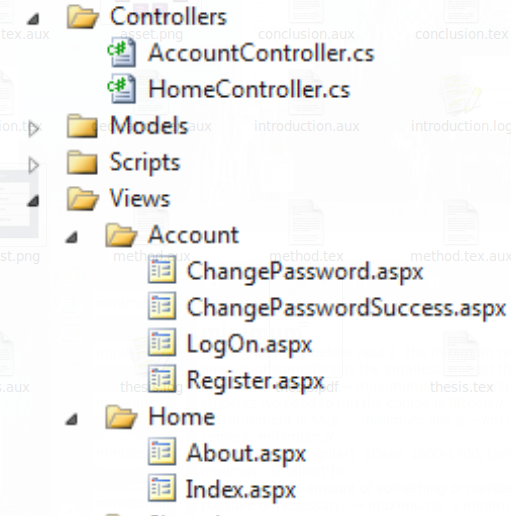
\includegraphics[scale=0.4]{URLRouting.png}
	\end{center}
	\caption{URL routing.}
\end{figure}
The Table~\ref{tab:routing} illustrates several typical URL routing examples.
\begin{table}[ht]
	\begin{center}
		\begin{tabular}{| l | c | c | c |}
			\hline
			URL & Controller Class & Action method & Passed parameter \\
			\hline
			/ & Home Controller & Index() & None \\
			\hline
			/Home & Home Controller & Index() & None \\
			\hline
			/Home/About & Home Controller & About() & None \\
			\hline
		\end{tabular}
		\caption{Examples of routing.}
		\label{tab:routing}
	\end{center}
\end{table}
The natural starting point to learn ASP.NET MVC is to understand the execution flow. The understanding of execution flow begins with the URL
routing.

With traditional web frameworks (classic ASP, PHP, ASP.NET Web Forms, etc), incoming URLs are typically mapped to files on disk.  For example: a 
request for a URL like ``/Books.aspx'' or ``/Books.php'' might be processed by a ``Books.aspx'' or ``Books.php'' file.

ASP.NET MVC includes a powerful URL routing engine that provides a lot of flexibility in controlling how URLs are mapped to controller classes.  It 
allows developers to completely customize how ASP.NET MVC chooses which controller class to create, which method to invoke on it, as well as configure
different ways that variables can be automatically parsed from the URL/Query string and passed to the method as parameter arguments.

By default, new ASP.NET MVC projects come with a pre-configured set of URL routing rules already registered.  This enables developers to easily get 
started on an application without having to explicitly configure anything. Routing configuration is loaded when the application starts. The default 
routing rule registrations can be found within the ``Application'' class of projects – which can be opened by double-clicking the ``Global.asax'' file
in the root of the project. This could be confirmed by setting one breakpoint on that line, and observe that this line is executed before any URL is 
interpreted.

This is one example of URL routing, based on the default routing rule, which is ``/{controller}/{action}/{id}'', where ``controller'' is the name of 
the controller class to instantiate, ``action'' is the name of a public method to invoke on it, and ``id'' is an optional parameter embedded within 
the URL that can be passed as an argument to the method. According the default rule, Controller = ``Home'', Action = ``Index'', and Id = ``'', if no 
argument is provided \cite{mvc_routing}.
\begin{figure}[h]
	\begin{center}
		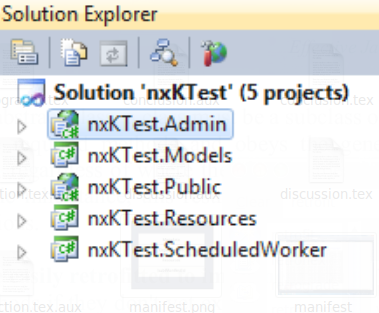
\includegraphics[scale=0.4]{application_layout.png}
	\end{center}
	\caption{Application Layout.}
	\label{fig:app_layout}
\end{figure}
\begin{figure}[t]
	\begin{center}
		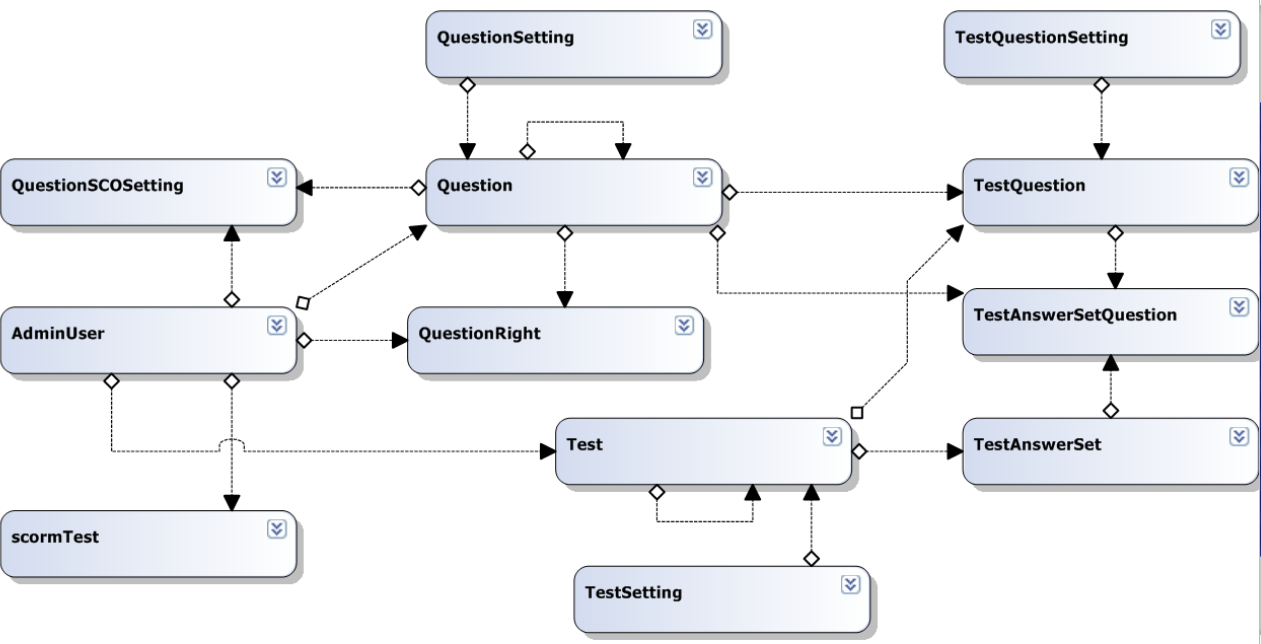
\includegraphics[scale=0.3]{database_layout.png}
	\end{center}
	\label{fig:database_layout}
	\caption{Table Relation Diagram.}
\end{figure}
\begin{figure}[h]
	\begin{center}
		\subfloat[Admin Project]{\label{fig:admin_project}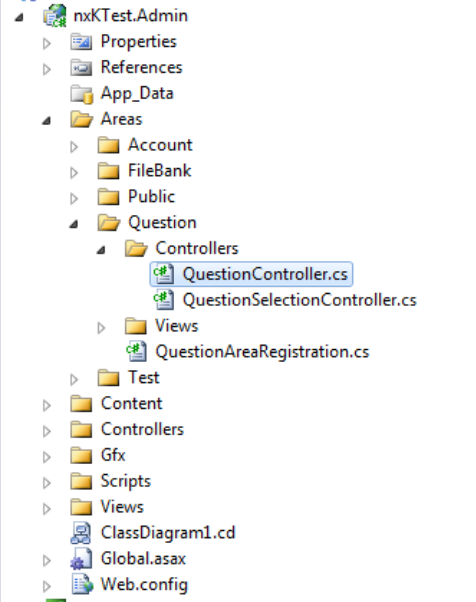
\includegraphics[scale=0.3]{admin_project.png}}
		\subfloat[Models Project]{\label{fig:models_project}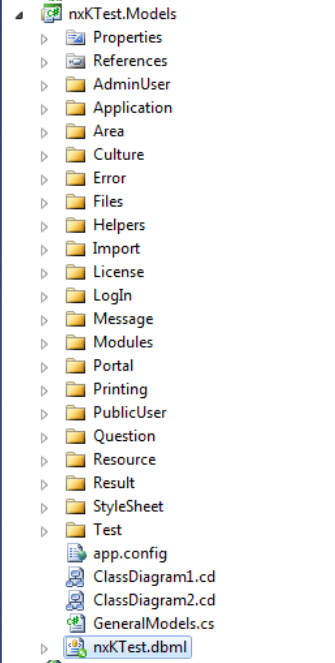
\includegraphics[scale=0.3]{models_project.png}}
		\subfloat[Public Project]{\label{fig:public_project}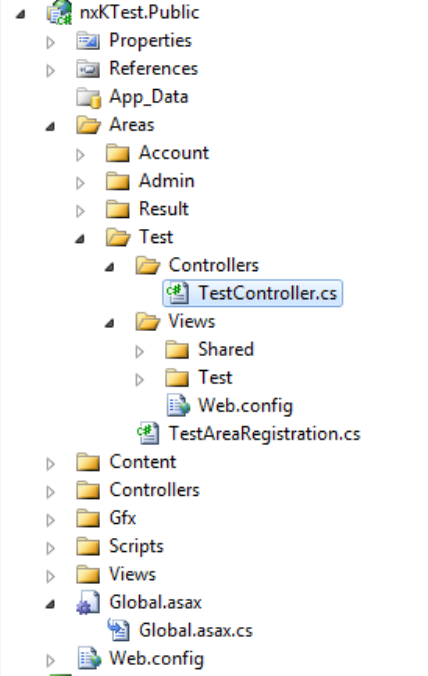
\includegraphics[scale=0.3]{public_project.png}}
	\end{center}
	\caption{Projects.}
\end{figure}
\subsection{nxtTest}
This application is divided into five projects, as showed in the Figure~\ref{fig:app_layout}. Only the first three will be used in this project. 
Since this project is the extension of one almost mature product, fully studying and understanding of it is critical before any non-trivial 
modification can be done. Consequently, the three projects are described briefly to illustrate how this project can be integrated into it.

The ``Admin'' project is responsible for the administration of LMS or tests. With proper right, users can create questions or import questions, create
tests by adding existing questions, and grade tests. The administrators of LMS can assign the right to users. The importing and exporting function 
belongs to this project. The file organization is shown in Figure~\ref{fig:admin_project}.

The ``Model'' project is the heart of this application, as is the heart of MVC architecture. A plethora of files exist in this project to reflect the 
various types of questions and tests. The file organization is shown in Figure~\ref{fig:models_project}. In this project, only a small subset is 
used.

The names of most tables are self-explaining, but some of them might be a little confusing.
QuestionSCOSetting is used to store the settings particularly for SCO questions; for SCO questions, the QuestionSetting is not much used. 

Tests are built out of questions, which will be saved in TestQuestion. The answers to tests are stored in TestAnswerSet. The relation between 
question and answer is stored in TestAnswerSetQuestion and TestAnswerSet, respectively. The reason for that is that sometimes the questions presented 
to users are randomly chosen from the question pool of the test.

QuestionRight is used to keep track of who has the right to use one particular question.

The ``Public'' project is where to see how the questions look like, which indicates that it is the interface to end users who are taking the tests, 
and question and test authors, who might want to have one preview of this question and test. The file organization is shown in 
Figure~\ref{fig:public_project}. The Launching functionality belongs to this project.
\section{Import whole package}
In the first case, import the package as one whole test, so that the LMS can launch it directly. Work needs to be done is to unzip this file,
and save the content to one folder. The name of this folder is generated as one Globally Unique Identifier(GUID), which can prevent users guessing 
what other tests exist in this LMS. SharpZipLib \cite{sharpziplib} is used to uncompress the zip file.

After uncompressing, several pieces of information need to be written to database: folder name(GUID), identifier(the attribute of manifest in 
imsmanifest.xml) and the name of the user importing this package. The reason for saving the identifier of this package is to prevent importing the
same package more than once.

According to SCORM 2004 standard \cite{cambook}, there is no guarantee that identifier is different from one to another. However, this attributes 
describe some information about this package, so it is reasonable to draw the conclusion that two packages with distinct content do not have the exact
same identifier. In addition, this project is the preliminary work; improvement can be made afterwards.

In the second case, all the SCOs in this package will be extracted so that course/test content developers could build tests using different 
combinations. In addition to what have been done for the first case, extra work needs to be taken, such as locating different SCOs and their 
associated information, save them at different directories, etc.
\begin{figure}[t]
	\begin{center}
		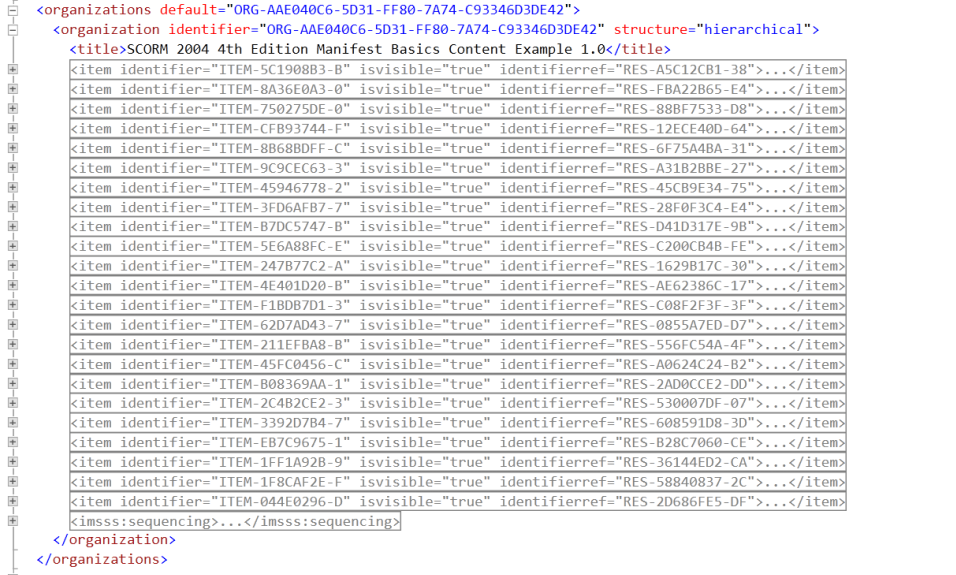
\includegraphics[scale=0.3]{manifest_organization.png}
	\end{center}
	\caption{Manifest organization.}
	\label{fig:organization}
\end{figure}
\begin{figure}[t]
	\begin{center}
		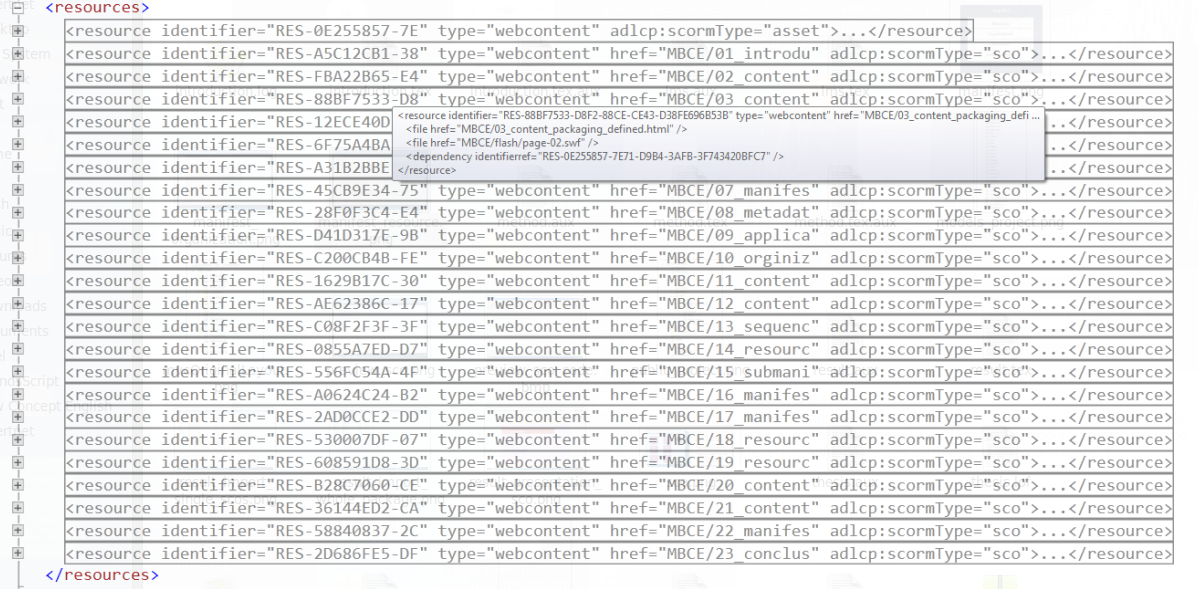
\includegraphics[scale=0.3]{manifest_resource.png}
	\end{center}
	\caption{Manifest resource.}
	\label{fig:resource}
\end{figure}
\section{Import single SCOs}
This package will be parsed in three phrases. Firstly, identify each SCO indicated in XML file. Secondly, identify all resources in this XML file. 
Finally, associate the resources with each SCO, copy the files to the appropriate locations, and save the information to the database.

In this project, Manifest Basics Content Example Content Package \cite{mbce_package} is used. In the highest level, two elements are of interest: 
\textless organizations \textgreater and \textless resources \textgreater. Figure~\ref{fig:organization} and Figure~\ref{fig:resource} is the 
screenshot of organization and resource of the manifest file in this package, respectively. These two work in parallel, constituting the whole 
package. When this manifest file is parsed, information concerning organization and resource is saved and their corresponding relation.

According to the content model, the \textless item \textgreater element represents an activity in the content organization. Therefore, in the first 
step, the \textless item \textgreater element in this XML file is kept track of, and associated with ``identifierref'' attribute, title, metadata 
information. The ``identifierref'' attribute works like one pointer, pointing to the resources this activity relies on.

One class called ``Item'' is created to save the information related to one item, and one Class called ``Items'' is created to keep track of all the 
items in this XML file, which works like one container.

In the second step, try to locate the resources indicated by ``identifierref'' in the previous step. Because of the existence of \textless dependency 
\textgreater element, the exact information what files constitute this resource is probably unknown when the ``xmlreader'' reach this point (It is 
possible that this resource depends on another resource, and that resource is defined way below this one). Therefore, keeping track of what resources 
exist in this XML file, and the content for each resource is necessary.

The implementation for resource is similar to above: ``Resource'' and ``Resources'' are created to save this information for later processing.

In the last step, ``interpret'' the resources, and figure out what files constitute each resource. The ``translation'' is done using recursion. The 
reason why recursion is used is that the level of including is unknown. In other words, it is possible that one resource depends on another resource, 
which depends on another resource, which depends on another resource, \ldots. Until now, the relation between SCO and its related files is 
established. The rest is clear; copy the related files to the fold represented by this SCO, and save the information to the database.

Specifically, the information will be saved to QuestionSetting table (even though there is not much to do, since the settings are stored in QuestionSCOSetting), Question, QuestionSCOSetting and QuestionRight tables.
\section{Exporting}
Exporting SCORM compliant package is the reverse of the above process, technically. Once the importing is fully understood, this section should be 
quite straightforward. This part is finished by Johan Simonsson from Entergate company.
\begin{figure}[t]
	\begin{center}
		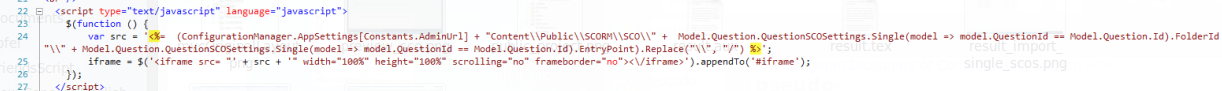
\includegraphics[scale=0.3]{preview_sco_code.png}
	\end{center}
	\caption{Code sample of PreviewSCORMQuestion.ascx}
	\label{fig:preview_sco_code}
\end{figure}
\section{Presenting Single SCO}
In this section, the work will be around ``Public'' project. One file named ``PreviewSCORMQuestion.ascx'' is responsible for the presentation of all 
the SCOs. Figure~\ref{fig:preview_sco_code} illustrates the content of it. The content of the SCO is inserted to one \textless iframe \textgreater 
using javascript for the presentation. Since the communication is not implemented for now, all the work is just to find the path to the entry point 
of the SCO from the database, and pass it to the javascript.
